% Benchmark C: closest-point (Gauss-point-to-segment) contact:
% slave Gauss point projected onto the closest master boundary segment
\documentclass[border=8pt]{standalone}
\usepackage{tikz}
\usetikzlibrary{arrows.meta}

\begin{document}
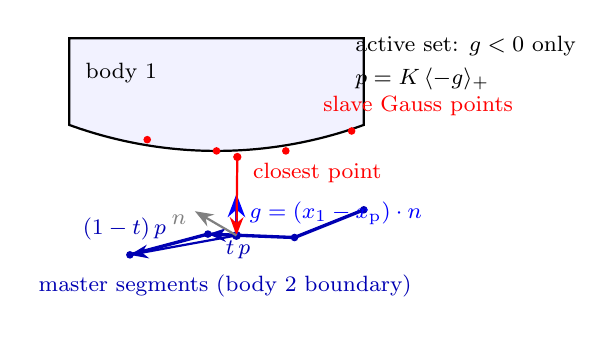
\begin{tikzpicture}[>={Stealth}, scale=2.2]

  % ---- body 1 bulk (slave body), drawn high with its boundary arc ----
  \draw[thick, fill=blue!5]
    (-0.35, 0.75) .. controls (0.2, 0.55) and (0.8, 0.55) .. (1.35, 0.75)
    -- (1.35, 1.25) -- (-0.35, 1.25) -- cycle;
  \node at (-0.05, 1.05) {\footnotesize body 1};

  % ---- slave Gauss points on the boundary arc ----
  \fill[red] (0.10, 0.665) circle (0.022);
  \fill[red] (0.50, 0.60) circle (0.022);
  \fill[red] (0.90, 0.60) circle (0.022);
  \fill[red] (1.28, 0.715) circle (0.022);
  \node[right, red, inner sep=4pt] at (1.05, 0.86)
    {\footnotesize slave Gauss points};

  % ---- master segments (body 2 boundary) ----
  \coordinate (m0) at (0.0, 0.0);
  \coordinate (m1) at (0.45, 0.12);
  \coordinate (m2) at (0.95, 0.10);
  \coordinate (m3) at (1.35, 0.26);
  \draw[very thick, blue!70!black] (m0) -- (m1) -- (m2) -- (m3);
  \foreach \p in {m0, m1, m2, m3} \fill[blue!70!black] (\p) circle (0.022);
  \node[below, blue!70!black, inner sep=4pt] at (0.55, -0.05)
    {\footnotesize master segments (body 2 boundary)};

  % ---- penetrating slave gp and its projection ----
  \fill[red] (0.62, 0.565) circle (0.024);
  \coordinate (proj) at (0.615, 0.112);
  \fill[blue!70!black] (proj) circle (0.026);
  % gap vector
  \draw[->, very thick, blue] (proj) -- ++(0.0, 0.24);
  \node[right, blue, inner sep=3pt] at (0.64, 0.24)
    {\footnotesize $g = (x_1 - x_{\mathrm{p}})\cdot n$};
  % projection line
  \draw[->, thick, red] (0.62, 0.565) -- (proj);
  \node[right, red, inner sep=3pt] at (0.66, 0.47)
    {\footnotesize closest point};

  % ---- force transfer to the two segment nodes ----
  \draw[->, thick, blue!70!black] (proj) -- (m0)
    node[pos=0.6, above left, inner sep=2pt] {\footnotesize $(1-t)\,p$};
  \draw[->, thick, blue!70!black] (proj) -- (m1)
    node[pos=0.6, below right, inner sep=2pt] {\footnotesize $t\,p$};

  % ---- normal vector n at the projection ----
  \draw[->, thick, gray] (proj) -- ++(-0.24, 0.14);
  \node[left, gray, inner sep=2pt] at (0.36, 0.2) {\footnotesize $n$};

  % ---- active set annotation ----
  \node[above right, inner sep=3pt, align=left] at (1.25, 0.9)
    {\footnotesize active set: $g<0$ only\\
     \footnotesize $p = K\,\langle -g\rangle_+$};

\end{tikzpicture}
\end{document}
